\documentclass[12pt]{ctexart}
\usepackage{amsfonts,amssymb,amsmath,amsthm,geometry,enumerate,graphicx}
\usepackage[colorlinks,linkcolor=blue,anchorcolor=blue,citecolor=green]{hyperref}
\usepackage[all]{xy}
%introduce theorem environment
\theoremstyle{definition}
\newtheorem{definition}{定义}
\newtheorem{theorem}{定理}
\newtheorem{lemma}{引理}
\newtheorem{corollary}{推论}
\newtheorem{property}{性质}
\newtheorem{proposition}{命题}
\newtheorem{example}{例}
\theoremstyle{plain}
\newtheorem*{solution}{解}
\newtheorem*{remark}{注}
\geometry{a4paper,scale=0.8}

\newcommand{\id}{\mathrm{id}}
\newcommand{\Aut}{\mathrm{Aut}}
\newcommand{\Inn}{\mathrm{Inn}}
\newcommand{\Orb}{\mathrm{Orb}}
\newcommand{\Stab}{\mathrm{Stab}}

\everymath{\displaystyle}

%article info
\title{\vspace{-2em}\textbf{环的概念}\vspace{-2em}}
\date{ }
\begin{document}
	\maketitle
	\begin{definition}[环]
		设集合$R$带有加法和乘法两种运算,满足
		\begin{enumerate}
			\item $R$对加法作成Abel群;
			\item $R$对乘法作成半群;
			\item 乘法对加法的左、右分配律成立,即对任意$a,b,m\in R$,有
			$$m(a+b)=ma+mb,\qquad (a+b)m=am+bm,$$
		\end{enumerate}
		则称$(R,+,\cdot)$是一个\textbf{环}.
	\end{definition}
	在环$R$中,将$R$对加法作成的群的单位元记作$0$,称为环$R$的\textbf{零元}.对任意$a\in R$,$a$在$R$对加法作成的群中的逆元记作$-a$,称为$a$的\textbf{负元}.
	\begin{definition}
		在环$R$中,对任意$m\in\mathbb{N}^+,a\in R$,定义
		$$ma=\underbrace{a+a+\cdots+a}_{m\text{个}},$$
	\end{definition}
	\begin{definition}
		由于环$R$对乘法作成半群,结合律成立,于是可以对任意$n\in\mathbb{N}^+,a\in R$,定义
	$$a^n=\underbrace{a\cdot a\cdot\cdots\cdot a}_{n\text{个}}.$$
	\end{definition}
	环中元素有一些基本的运算性质.对任意$a\in R,m,n\in\mathbb{N}^+$,有
	$$(m+n)a=ma+na$$
	$$m(-a)=-ma$$
	$$(mn)a=m(na)$$
	$$m(a+b)=ma+mb$$
	
	$$a^ma^n=a^{m+n}$$
	$$(a^m)^n=a^{mn}$$
	且
	$$\left(\sum_{i=1}^{m}a_i\right)\left(\sum_{j=1}^{n}b_j\right)=\sum_{i=1}^{m}\sum_{j=1}^{n}a_ib_j=\sum_{j=1}^{n}\sum_{i=1}^{m}a_ib_j.$$
	对$0,a,b\in R$,有$0a=a0=0$,$(-a)b=a(-b)$,$(-a)(-b)=ab$.
	
	环$R$对乘法并不作成群,乘法逆元不一定存在,于是消去律不一定满足,于是有零因子的定义.
	\begin{definition}[零因子]
		设$R$是环,$a,b\in R$且$a,b\neq 0$,若$ab=0$,则称$a$为$R$的\textbf{左零因子},$b$为$R$的\textbf{右零因子}.$a$和$b$都简称为$R$的\textbf{零因子}.
	\end{definition}
	\begin{definition}[交换环]
		乘法交换的环为\textbf{交换环}.
	\end{definition}
	\begin{definition}[幺环]
		对乘法作成幺半群的环为\textbf{幺环}.
	\end{definition}
	\begin{definition}[无零因子环]
		没有零因子的环称为\textbf{无零因子环}.
	\end{definition}
	\begin{definition}[整环]
		无零因子的交换幺环称为\textbf{整环}.
	\end{definition}
	\begin{definition}[体]
		非零元可逆的无零因子幺环,即非零元对乘法构成群的环称为\textbf{体}.
	\end{definition}
	\begin{definition}[域]
		非零元可逆的整环,即乘法交换的体称为\textbf{域}.
	\end{definition}
	它们的关系如下.
	\begin{figure}[htbp]
		\centering
		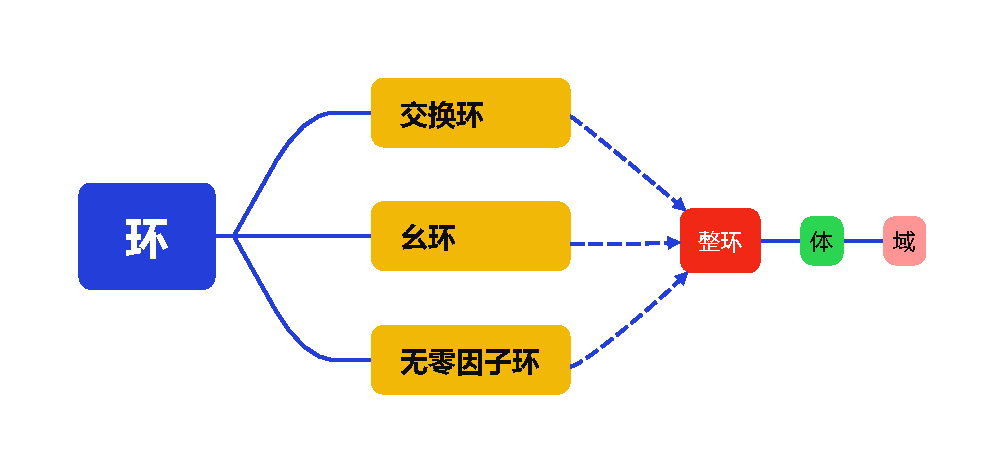
\includegraphics[width=15cm]{mindmap.pdf}
		\caption{几种环的关系示意图}
	\end{figure}
	\begin{definition}[子环]
		设$R$是环,若它的非空子集$R_1$对环$R$的加法和乘法也构成环,则称$R_1$是$R$的\textbf{子环}.
	\end{definition}
	\begin{definition}[理想]
		设$I$是$R$的子环,若对任意$a\in I$,$r\in R$,有$ra\in I$,则称$I$为$R$的\textbf{左理想}.若对任意$a\in I$,$r\in R$,有$ar\in I$,则称$I$为$R$的\textbf{右理想}.若$I$既是$R$的左理想,又是$R$的右理想,则称$I$是$R$的\textbf{双边理想},简称\textbf{理想},记作$I\lhd R$.
	\end{definition}
	环本身和$\{0\}$都是理想,称为\textbf{平凡理想}.
	\begin{theorem}[子环的充要条件]
		设$R$是环,$R_1$是$R$的非空子集,则$R_1$是$R$的子环当且仅当对任意$a,b\in R_1$,有$a-b\in R_1,ab\in R_1$.
	\end{theorem}
	\begin{proof}
		必要性:若$R_1$是$R$的子环,则$R_1$对加法作成交换群,于是$R_1$是$R$关于加法的子群.由子群的充要条件,对任意$a,b\in R_1$,有$a-b\in R_1$.而$R_1$构成环,于是关于乘法作成半群,运算封闭.对任意$a,b\in R_1$,有$ab\in R_1$.
		
		充分性:若对任意$a,b\in R_1$,有$a-b\in R_1$,$a,b\in R_1$,则由子群的充要条件,$R_1$对加法作成$R$的子群,自然继承$R$中加法的交换性,于是对加法作成交换群.而乘法继承$R$中的结合性,又因为对任意$a,b\in R_1$,$ab\in R_1$满足封闭性,关于乘法作成半群.在$R_1$中,继承$R$的分配律,对任意$a,b,c\in R_1$,$a(b+c)=ab+ac,(a+b)c=ac+bc$,于是$R_1$是$R$的子环.
	\end{proof}
	\begin{corollary}[理想的充要条件]
		设$R$是环,$I$是$R$的非空子集,则$I$是$R$的理想当且仅当对任意$a,b\in I$,任意$x,y\in R$,有$a-b\in R_1,xa,ay\in R_1$.
	\end{corollary}
	\begin{definition}[商环]
		设$R$是环,$I\lhd R$,在$R$中定义关系$a\sim b\iff a-b\in I$,则关系$\sim$对环的加法和乘法为同余关系.记$a\in R$所在的等价类为$a+I$,在商集合$R/I$上定义运算
		$$(a+I)+(b+I)=(a+b)+I,$$
		$$(a+I)(b+I)=ab+I.$$
		则$R/I$对上述运算作成环,称为$R$对$I$的\textbf{商环}.
	\end{definition}
	\begin{proof}
		首先证明$\sim$是同余关系.先证明它是等价关系.
		
		反身性:任意$a\in R$,$a-a=0\in I$,于是$a\sim a$.
		
		对称性:对任意$a,b\in R$,若$a\sim b$,则$b-a=-(a-b)\in I$,于是$b\sim a$.
		
		传递性:对任意$a,b,c\in R$,若$a\sim b,b\sim c$则$a-c=(a-b)+(b-c)\in I$,于是$a\sim c$.
		
		于是$\sim$是等价关系.对任意$a,a_1,b,b_1\in R$,若$a\sim b$,$a_1\sim b_1$,则
		$$(a+a_1)-(b+b_1)=(a-b)+(a_1-b_1)\in I\quad\Rightarrow\quad (a+a_1)\sim(b+b_1),$$
		$$aa_1-bb_1=aa_1-ab_1+ab_1-bb_1=a(a_1-b_1)+b_1(a-b)\in I\quad\Rightarrow\quad aa_1\sim bb_1,$$
		于是$\sim$对加法和乘法都成同余关系.
		
		然后证明$R/I$是环.
		
		封闭律:对任意$a+I,b+I\in R/I$,
		$$(a+I)+(b+I)=(a+b)+I\in R/I,$$
		$$(a+I)(b+I)=ab+I\in R/I,$$
		
		结合律:对任意$a+I,b+I,c+I\in R/I$,
		\begin{equation*}
			\begin{aligned}
				&\left[(a+I)+(b+I)\right]+(c+I)=(a+b)+I+(c+I)=((a+b)+c)+I\\
				&=(a+(b+c))+I=a+I+(b+c)+I=a+I+\left[(b+I)+(c+I)\right].
			\end{aligned}
		\end{equation*}

		$$\left[(a+I)(b+I)\right](c+I)=(ab+I)(c+I)=(ab)c+I=a(bc)+I=(a+I)\left[(b+I)(c+I)\right].$$
		
		加法幺元:$0+I$,对任意$a+I\in R/I$,
		$$(a+I)+(0+I)=(a+0)+I=a+I.$$
		
		加法逆元:对任意$a+I\in R/I$,
		$$(a+I)+(-a+I)=(a-a)+I=0+I.$$
		
		加法交换律:对任意$a+I,b+I\in R/I$,
		$$(a+I)+(b+I)=(a+b)+I=(b+a)+I=(b+I)+(a+I).$$
		
		分配律:对任意$a+I,b+I,c+I\in R/I$,
		\begin{equation*}
			\begin{aligned}
				&(a+I)\left[(b+I)+(c+I)\right]=(a+I)((b+c)+I)=a(b+c)+I\\
				&=(ab+ac)+I=(a+I)(b+I)+(a+I)(c+I).
			\end{aligned}
		\end{equation*}
		\begin{equation*}
			\begin{aligned}
				&\left[(a+I)+(b+I)\right](c+I)=((a+b)+I)(c+I)=(a+b)c+I\\
				&=(ac+bc)+I=(a+I)(c+I)+(b+I)(c+I).
			\end{aligned}
		\end{equation*}
		于是$R/I$对上述的加法和乘法作成环.
	\end{proof}
	\begin{remark}
		这里关系用符号“$\sim$”表示,从而不会与环$R$混淆.证明过程中,等价类的运算,最后归结为代表元的运算.
	\end{remark}
\end{document}